Este trabalho se trata de um estudo de caso, pois se avalia o \textit{Lean Learning} em um contexto da vida real, com finalidade de pesquisa empírica, visando aprofundar os estudos na área \cite{MIGUEL2007}. Além disso, não há aprioristicamente um esquema estrutural já elaborado, não tendo um problema e variáveis previamente definidas, portanto seu objetivo é apreender determinada situação e descrever o caso observado \cite{marconi2003fundamentos} \cite{marconi2012tecnicas}. Devido a essas características, este estudo de caso também assume caráter exploratório, uma vez que tem o objetivo de estudar uma ideia ou intuição ainda pouco explorada \cite{de2011metodologia} a partir da literatura existente e avaliar hipóteses com base nas descobertas feitas.

A pesquisa envolve medidas qualitativas, como a satisfação dos alunos e dos professores com as atividades propostas com o \textit{Lean Learning} e gera métricas quantitativas \cite{Metricas} para análise geral dos resultados obtidos, como indicadores de satisfação, adequação e proximidade com o mercado de trabalho, para cada uma das atividades realizadas. Como objeto de estudo do trabalho tem-se a etapa \textit{Measure} (Medir) do \textit{Lean Learning}.

A seguir encontram-se detalhados os procedimentos que foram executados no estudo, conforme Figura 2, visando a obtenção dos resultados que possibilitam extrair conclusões do fenômeno estudado.

\begin{figure}[!ht]
    \centering
    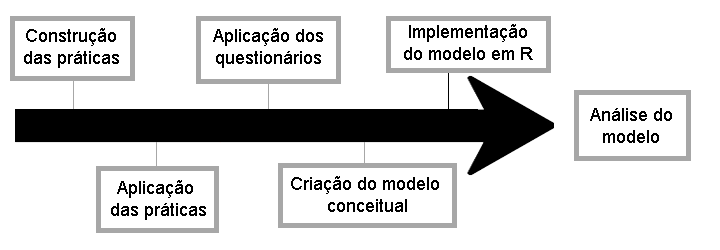
\includegraphics[width=15cm,height=5cm]{Imagens/Procedimento.png}
    \caption{Procedimentos. Fonte: autores}
    \label{fig:Procedimento}
\end{figure}

\subsection{Construção das atividades práticas}

Neste trabalho estuda-se a etapa de Medir, do \textit{Lean Learning}. Para isso, foram propostas atividades práticas que foram acompanhadas pelos autores deste trabalho e serviram como protótipos no desenho do processo. Essas atividades são: 

    \begin{enumerate}\setlength\itemsep{0.5em}
        \item Prática envolvendo compreensão e refinamento de requisitos de \textit{software}.
        \item Prática envolvendo trabalho em equipe, velocidade e competitividade.
        \item Prática envolvendo trabalho em equipe, \textit{brainstorming}, criatividade e comunicação.
    \end{enumerate}

Na prática 1 foi proposto que os alunos se organizassem em trios. Um dos três elaborou requisitos para uma tela de um sistema de sua escolha. Apenas através de texto, os requisitos da tela foram descritos e passados para os outros dois alunos. Ao receberem os requisitos, os dois ilustraram uma tela, na ferramenta de sua escolha, de acordo com as especificações dadas, de forma individual. Ao final da elaboração das telas, houve uma reflexão com os alunos mediada pelos pesquisadores, sobre o que se esperava na tela e porque a tela foi feita daquela maneira. Foi possível analisar pontos da etapa da elicitação de requisitos, como a fragilidade de requisitos ambíguos ou mal descritos e também como a interpretação dos requisitos pode alterar o resultado. Para essa atividade prática foram concedidos aproximadamente 30 minutos de aula.

Na prática 2 uma lista contendo 4 problemas de programação foi apresentada aos alunos, que tiveram de se organizar em grupos de 3 ou 4 integrantes. Durante 30 minutos eles resolveram o máximo de problemas que conseguiram, podendo se organizar segundo seus próprios critérios -- decidindo como seria a divisão de tarefas entre os membros, quais linguagens, recursos e ferramentas seriam utilizados etc. Essa prática impôs quatro restrições: 
    \begin{enumerate}\setlength\itemsep{0.5em}
        \item Os alunos teriam apenas 30 minutos para a resolução dos problemas;
        \item Todos os integrantes dos grupos deveriam atuar na resolução dos problemas (ou seja, nenhum deveria ficar ocioso);
        \item Todos os grupos formados deveriam operar de forma individual, não podendo haver cooperação entre eles;
        \item Ao final do tempo dedicado à resolução dos problemas, os alunos deveriam entregar um arquivo compactado contendo todas as soluções, de modo a garantir que nenhum código fosse alterado após o prazo.
    \end{enumerate}
Para avaliar a resolução dos problemas, foram verificados apenas os conjuntos de saídas para cada conjunto de entradas testado, desconsiderando a implementação adotada no código. O critério de desempate, caso houvesse, foi ordem de entrega. Essa atividade visa estimular trabalho em equipe, agilidade, coordenação e uma competição saudável entre os alunos. De modo a estimular a competição, foi negociada a possibilidade de dar pontos extras (até 2) como prêmio aos membros da equipe vencedora, em cada disciplina em que a prática foi aplicada. Para essa atividade prática foram concedidos aproximadamente 30 minutos de aula. Os problemas de programação encontram-se no apêndice deste trabalho. 

Na prática 3, os alunos de toda a turma foram considerados um só grupo. Foi apresentado um vídeo com o título ``Os problemas da educação atual."\footnote{Link do vídeo: https://www.youtube.com/watch?v=bopmvB6a5Ls\&ab\_channel=ProjetoEducatuX}, do canal ``Projeto EducatuX"\ e esse vídeo serviu como base principal da prática. Os alunos deveriam chegar a um consenso sobre qual foi o problema principal abordado no vídeo e propor uma solução em modelo de \textit{software} para tal problema. Também foi requisitado que citassem e explicassem 4 requisitos funcionais e 2 requisitos não funcionais do modelo proposto pelos mesmos. Essa prática visa exercitar o trabalho em equipe e a comunicação com um grande número de pessoas, além de estimular a criatividade para solução de problemas. Para essa atividade prática foram concedidos aproximadamente 30 minutos de aula. Nessa prática deveriam ser gerados os seguintes artefatos:
\begin{itemize}\setlength\itemsep{0.5em}
    \item Uma descrição do problema abordado no vídeo.
    \item Uma descrição de um \textit{software} que auxilie na solução do problema.
    \item Lista de requisitos do \textit{software} descrito anteriormente.
\end{itemize}
Todos os artefatos deveriam ser postados em um formulário do \textit{Google Forms} e então os pesquisadores poderiam analisar as ideias propostas. Essa prática possui várias soluções possíveis e não há solução certa ou competição, visto que todos os alunos deveriam colaborar visando um mesmo objetivo, a partir de suas perspectivas\nocite{VideoPrat3}.

Para manter a consistência dos resultados, as práticas foram aplicadas em disciplinas que estão ligadas aos seus temas. As disciplinas nas quais o experimento foi realizado são: Algoritmos e Estruturas de Dados, Engenharia de Requisitos, Arquitetura de \textit{Software}, Medição e Experimentação em Engenharia de \textit{Software} e Gestão da Produção de \textit{Software}. 

\subsection{Aplicação das atividades práticas}

Os professores das disciplinas citadas anteriormente foram contatados pelos autores e concordaram em ajudar na experimentação da metodologia durante um período letivo em sua respectiva disciplina. A escolha dos professores foi baseada em: i) relação da sua disciplina com processos de desenvolvimento de \textit{software} ou gestão \textit{Lean} e ii) período em que a disciplina está alocada no curso. 

A seleção das disciplinas foi abrangente, visando introduzir e discutir temas que seriam novidade para os alunos dos primeiros períodos da graduação e também revisitar temas já estudados e consolidados com os alunos dos períodos mais avançados. Essa abrangência foi pensada para tentar obter respostas diversificadas, dada a diferença de experiência entre os participantes, não só em relação ao próprio curso, mas também em relação ao mercado de trabalho. As práticas foram executadas entre 10 de março e 29 abril de 2021, em aulas que ocorriam via \textit{Microsoft Teams}, durante o Regime Letivo Remoto, adotado no contexto da pandemia do vírus COVID-19. 

A etapa Medir utiliza das atividades práticas para gerar os dados que são analisados e servem como \textit{feedback} para os pesquisadores e também para o professor, que é o agente central no \textit{Lean Learning}. A partir das métricas obtidas, torna-se possível medir o benefício dessas práticas no ensino e também identificar pontos de melhoria nas mesmas, buscando a melhoria contínua pregada pela metodologia. Ao final de cada prática, foram coletadas as percepções dos alunos e professores participantes acerca do que foi exercitado. A coleta desses dados foi feita por meio da aplicação de questionários do \textit{Google Forms} (contidos no Apêndice).

\subsection{Aplicação dos questionários}

O uso de questionários como instrumentos para coleta e análise de dados é apontado em dois trabalhos, sendo eles o de Bandeira (2003)\nocite{Questionarios1} e de Henkel (2017)\nocite{Questionarios2}. Foram aplicados três questionários diferentes aos participantes: dois aos alunos e um aos professores. A aplicação se repetiu a cada prática finalizada, pois o objetivo era verificar a opinião de ambas as partes sobre todas as práticas de forma individual. A descrição do conteúdo e da finalidade de cada questionário encontra-se nas Subseções 4.3.1, 4.3.2 e 4.3.3.

\subsubsection{Questionário fechado dos professores}

É utilizado um questionário fechado destinado aos professores, contendo questões que contemplam suas percepções de: i) engajamento dos alunos em relação a atividade prática; ii) complexidade da prática realizada; iii) desempenho dos alunos na atividade proposta; iv) fixação do conhecimento pela atividade; v) proximidade entre a prática e demandas do mercado. As opções de resposta para cada pergunta estão organizadas em escala Likert de cinco pontos. Devido ao baixo número de respostas, pois são apenas seis professores, foi feita apenas uma análise descritiva de suas respostas.

\subsubsection{Questionário fechado dos alunos}

Esse questionário contém questões de triagem e questões de pesquisa. As questões de triagem visam entender melhor quem é o respondente, coletando os seguintes dados: i) se é aluno da Engenharia de \textit{Software}; ii) sexo biológico; iii) faixa etária; iv) período da graduação em que se encontra; v) há quanto tempo trabalha na área. As questões de pesquisa abordam: i) satisfação com a participação na atividade prática; ii) percepção do nível de adequação da prática ao contexto em que ela foi aplicada; iii) percepção do nível de proximidade da prática com o mercado de trabalho de \textit{software}. Para medir as respostas com base em cada um desses três tópicos, foram feitas três perguntas para cada, totalizando nove perguntas de pesquisa. Cada pergunta de pesquisa apresenta opções de resposta baseadas em escala Likert de cinco pontos.

Os três tópicos que contém as nove questões de pesquisa servem para gerar três variáveis: Satisfação (S), Adequação (A) e Proximidade com o mercado de trabalho (M). Essas variáveis são discutidas e detalhadas na Subseção 4.4.

Em ambos os questionários fechados, o uso da escala tipo Likert de cinco pontos possibilitou a obtenção de uma graduação quantificada das percepções dos respondentes \cite{marconi2003fundamentos}. Seu maior benefício é conseguir medir, de forma graduada, graus de concordância ou não em relação a um conjunto de sentenças.

\subsubsection{Questionário aberto dos alunos}

O questionário aberto dos alunos visa a obtenção de: i) percepções dos alunos não contempladas no questionário fechado; ii) \textit{feedbacks} de possíveis melhorias nas práticas. As respostas obtidas precisam ser interpretadas e simplificadas a tópicos principais abordados nelas, para então se realizar uma análise de tópicos e verificar convergências, de modo a identificar e agrupar opiniões.

Com as respostas obtidas, foi conduzida a fase de análise de dados. Na Subseção 4.4 encontra-se a discussão do modelo conceitual que foi elaborado para fazer as medições e análises sobre o questionário fechado dos alunos, que é central neste trabalho. Os demais questionários foram analisados segundo detalhes contidos em sua descrição nesta mesma subseção.

\subsection{Criação do modelo conceitual e validação implementada em R}

Foi criado um modelo conceitual para medir a efetividade da aplicação de praticas no ensino. O modelo pode ser visto abaixo, na Figura 3.  

\begin{figure}[!ht]
    \centering
    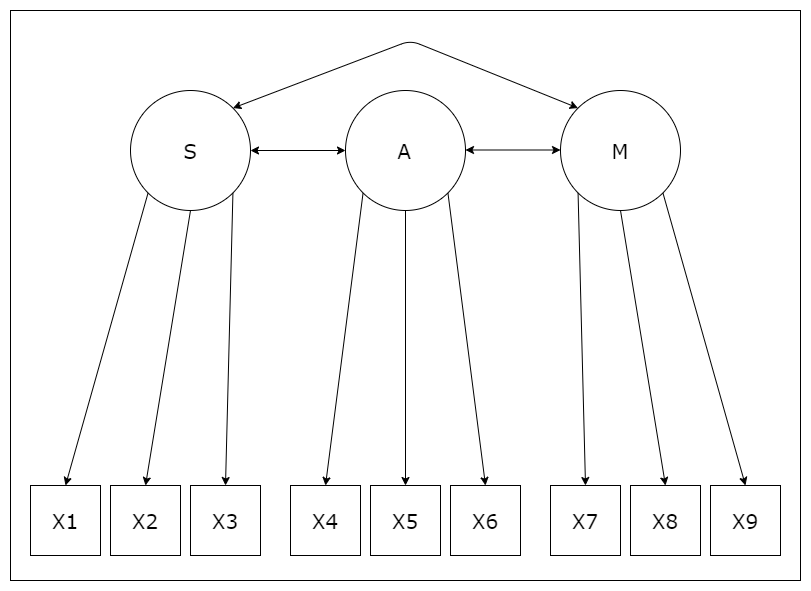
\includegraphics[width=12cm,height=8.6cm]{Imagens/ModeloConceitualTCC.png}
    \caption{Modelo conceitual. Fonte: autores}
    \label{fig:ModeloConceitualTCC}
\end{figure}

A validação do modelo conceitual foi baseada em Análise Fatorial Confirmatória e sua implementação feita através de um \textit{script} na linguagem de programação R\footnote{Site oficial da linguagem: https://www.r-project.org/about.html}, via RStudio\footnote{Site oficial do IDE: https://www.rstudio.com/} (versão 1.4.1103), utilizando a biblioteca \textit{lavaan}\footnote{Site oficial da biblioteca: https://lavaan.ugent.be/} (\textit{latent variable analysis}), de análise de variáveis latentes. As variáveis latentes deste trabalho são as mesmas mencionadas anteriormente: Satisfação (S), Adequação (A) e Proximidade com o mercado de trabalho (M). Cada uma é medida a partir de três variáveis observadas específicas (vide Subseção 4.3.2). A notação matemática para obter os valores das variáveis latentes a partir das observadas é a seguinte:

$S = \beta_{0S} + \beta_{1S}X_{1} + \beta_{2S}X_{2} + \beta_{3S}X_{3} + \epsilon_{1S}$

$A = \beta_{0A} + \beta_{1A}X_{4} + \beta_{2A}X_{5} + \beta_{3A}X_{6} + \epsilon_{1A}$

$M = \beta_{0M} + \beta_{1M}X_{7} + \beta_{2M}X_{8} + \beta_{3M}X_{9} + \epsilon_{1M}$

Onde $X_{1}$ a $X_{9}$ representam as nove variáveis observadas, contendo valores obtidos através das respostas ao questionário fechado dos alunos. A função \textit{cfa()} do pacote \textit{lavaan} é uma função específica para a análise de modelos fatoriais confirmatórios, gerando automaticamente a variância e covariância das variáveis observadas e latentes, além de estimar o valor do intercepto e do erro residual.

A avaliação da validade dos constructos foi feita com base em confiabilidade. A confiabilidade indica o nível em que os itens operacionais dos construtos latentes são consistentes e confiáveis em suas métricas \cite{hair2005fundamentos}. Os indicadores utilizados para tal foram o Alfa de Cronbach e Confiabilidade Composta \cite{chin1998commentary}. Tanto o Alfa de Cronbach quanto a Confiabilidade Composta devem apresentar valores acima de 0,60, no caso de pesquisas exploratórias \cite{hair2005fundamentos} como esta. Carga Fatorial pode ser definida como a métrica que indica o quanto uma variável é explicada pelos seus fatores, além de permitir o entendimento do comportamento de um fenômeno \cite{hair2005fundamentos}. A discussão dos resultados se encontra na Seção 5.